\documentclass{article}

\usepackage{ctex}
\usepackage{graphicx}
\usepackage{float}
\usepackage{datetime}
\usepackage{hyperref}
\usepackage{amssymb}
\usepackage{amsthm}
\newtheorem{theorem}{Theorem}
\newtheorem{corollary}{Colollary}
\newtheorem{lemma}{Lemma}
\newtheorem{definition}{Definition}
\renewcommand\proofname{Proof}
\renewcommand\figurename{Figure}
\usepackage{listings}
\usepackage{xcolor}

\title{CS216 Assignment2 \\ {\begin{large} Solve DMST Problem in $O(m\log n)$ Time\end{large}}}

\author{匡亮(12111012)}

\date{March 24, 2023}

\begin{document}

\maketitle

\renewcommand\abstractname{Abstract}
\begin{abstract}

This is my report of CS216 Assignment2, including:

\begin{itemize}
    \item[1.] What the Directed Minimum Spanning Tree problem is.
    \item[2.] How Edmond's Algorithm solves this problem and how Tarjan's implementation improves it to $O(m\log n)$.
    \item[3.] A sample code in C++ and detailed time complexity analysis.
    \item[4.] A little expansion.
\end{itemize}

\end{abstract}

\newpage

\renewcommand\contentsname{Contents}
\tableofcontents

\newpage

\section{Problem Definition}

Let $G=(V,E,w)$ be a weighted directed graph, where $w:E\to\mathbb{R}$ is the cost function. Let $r\in V$. A directed spanning tree (DST) of G rooted at $r$, is a subgraph $T$ of $G$ such that the undirected version of $T$ is a tree and $T$ contains a directed path from $r$ to any other vertex in $V$. The one with the minimum total cost is called the minimum directed spanning tree (MDST). The problem is to find a MDST on a given graph $G$ and a given root $r$.

For convenience, in the whole report we assume $|V|=n,|E|=m$ $O(\log m)=O(\log n)$.

\section{Algorithm}

\subsection{Important lemma}

The whole algorithm is based on a subtle lemma.

\begin{lemma}
    For each vertex $v\in V/\{r\}$, let $e_v$ be the entering edge of $v$ with minimum cost, and let $E'$ be the edge set of all $n-1$ different $e_v$, then:
    \begin{itemize}
        \item [1.] If there is no rings in $E'$, then $E'$ is the MDST.
        \item [2.] Otherwise, for each circle $C_i\in E'$, there is a MDST containing $|C_i|-1$ edges in $C_i$.
    \end{itemize}
\end{lemma}

\begin{proof}
    The first one is trival. We need an entering edge for each vertex except $r$, and fortunately we independently minimized each of them, then we literally get the MDST.

    For the second one, it is trival for the case $|C|=1$. Otherwise, let the circle $C=v_1\to v_2\to...\to v_k\to v_1$ and W.L.O.G let $v_1$ be one of the closest vertices to $r$ on the circle, i.e. there is not an ancestor of $v_1$ in $C$ (note that the edge $(v_k,v_1)\not\in T$). Assume that $e_{v_{i+1}}=(v_i,v_{i+1})\not\in T, 1\le i<k$ is the \textbf{first} edge on $C$ (which means $i$ is minimized) that is not in $T$, while $e'=(u,v_{i+1})\in T$ for some other vertex $u$. Then, $u$ and $v_{i+1}$ are not ancestors of $v_1$, and $v_1$ is the ancestor of $v_2,v_3,...,v_i$, then $u$ and $v_{i+1}$ are not ancestors of $v_i$. Therefore we can force $v_i$ to be the parent of $v_{i+1}$ with out forming a circle. Then, $T'=T/\{e'\}\cup\{e_{v_i}\}$ is also a MDST, because $T'$ is a DST and $w(e_{v_{i+1}})\le w(e')$.

    We can repeat the method above until the MDST we maintain contains $|C_i|-1$ edges in $C_i$ for each circle $C_i\in E'$.
\end{proof}

\begin{figure}
    \centering
    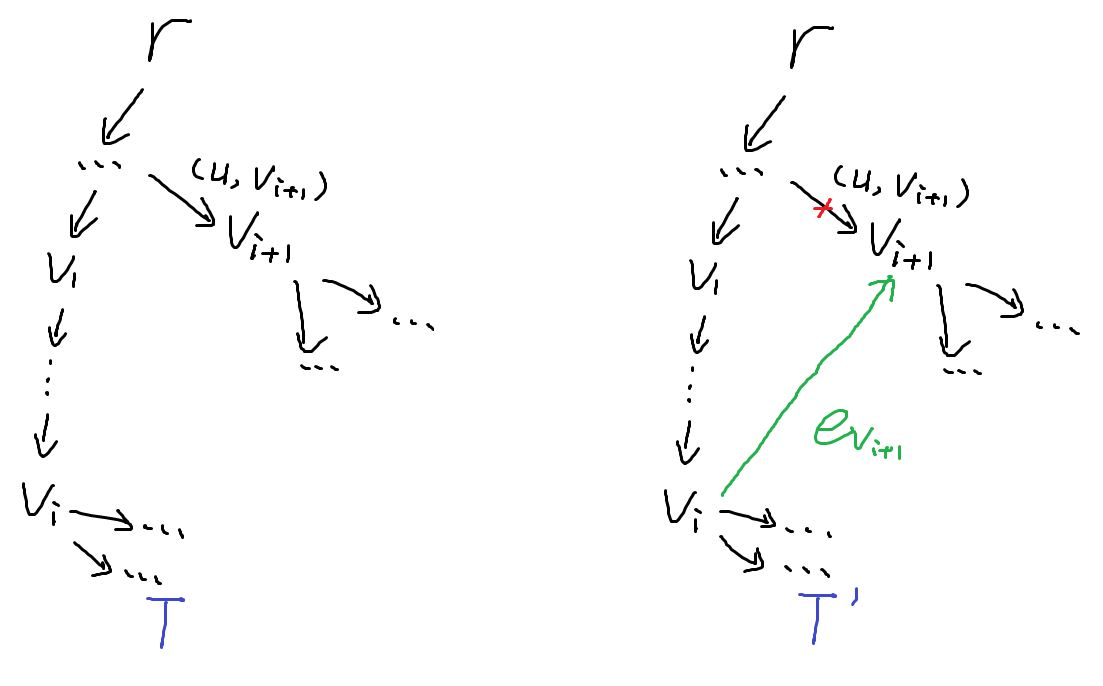
\includegraphics[height=7cm,width=11cm]{figure/figure1.png}
    \caption{graphic explanation for the proof above}
    \label{1}
\end{figure}

With the lemma above, our basic idea is that we maintain the set $E'$, and think what we should do when we find a circle.

\subsection{Algorithm - Contract part}

If we find no circles, we complete the problem. So if we find a circle, insteadly, let's try to \textbf{reduce the scale of the problem}.

With the lemma above, when we find a circle, we know that we can always retain all except one of the circle edges. Therefore, we no longer need the edges between the vertices on the circle, and only care about from which vertex we enter the circle on the final MDST (we can know from which we exit at the same time). With this idea, we can contract a circle into a super-vertex. As we need all except one of circle edges, we add the total cost of circle edges to our final result (total weight of MDST, if you do not care, just skip this step), and minus $w(e_v)$ from the weight of all edges entering $v$ for all $v$ on the circle we found. Then when we chose an edge to enter the circle at some vertex $v_0$ later, we automatically remove $e_{v_0}$ from our answer.

This method can benefit our work from many aspects. Firstly, we do not need to differentiate between vertex and super-vertex during the process. Secondly, if the graph is strongly connected, we do not care about what $r$ is, because we will always get a single super-vertex contain all vertices in the end. So we can add edges $(1,2),(2,3),...,(n,1)$ with weight $INF$ to the graph to make sure it is strongly connected and not influence the result, where $INF$ is a constant big enough, like $INF=\sum_{e\in E}w(e)$. Thirdly, instead of maintaining a DST or a set of edges, we can easily maintain a chain, and try to add $e_v$ of the graph \textbf{now} where $v$ is the head of the chain (recall that $e_v$ means the entering edge of $v$ with minimum cost), and detect that whether we have formed a circle by adding this edge or not.

Finally, what we need to do in this part is:

\begin{itemize}
    \item [1.] Add $n$ auxiliary edges.
    \item [2.] Pick an arbitrary vertex $a$ as the head of the chain we maintain to begin.
    \item [3.] If $e_a$ does not exist, we have finished. Otherwise, get $e_a\leftarrow(u,v)$.
    \begin{itemize}
        \item [3.1] If it is inside the super-vertex $a$, ignore it.
        \item [3.2] If $u$ is a new vertex, we extend our chain by set $a\leftarrow u$.
        \item [3.3] Otherwise, we formed a circle. We set a new super-vertex $c$ to include all the vertices on the circle, and for each vertex $v$, minus the weight of its \textbf{entering circle edge} (not $e_v$) from all edges entering it, and set $parent[v]\leftarrow c$. Finally we maintain our chain by set $a\leftarrow c$
    \end{itemize}
    \item [4.] Repeat \textbf{step 3.} .
\end{itemize}

Natually, we want to use a data structure on each vertex to maintain its entering edges. We need it to do the following things:

\begin{itemize}
    \item [1.] Get the minimum value of a set and delete it.
    \item [2.] Minus a constant from all values in a set.
    \item [3.] Merge two sets.
\end{itemize}

\textbf{Leftist Heaps} with lazy-tag trick can do the jobs above in $O(\log n)$ time, which we will introduce later.

Also, we need a data structure to tell us which super-vertex each vertex is in now, because in step \textbf{3.3}, we only know $e_a=(u,v)$, but $u$ may be not on the chain now, a super-vertex containing $u$ insteadly is. This can be done by \textbf{Disjoint Set Union} in $O(\log n)$ time (it can be faster but $O(\log n)$ is enough here).

\subsection{Algorithm - Expand part}

Now, we have a super-vertex containing all vertices and other inside layer super-vertices. We need two very simple functions to call each other and finish the task.

\subsubsection{Expand a vertex}

We use $ExpandVertex(v,r)$ to calculate the sub-question in a super-vertex $r$ with entering vertex $v$, where $v$ is one of the $n$ original vertices. We know that $v$ is the entering vertex of $parent[v]$'s circle, $parent[v]$ is the entering vertex of $parent[parent[v]]$'s circle, and so on. So for each layer, we call another function $ExpandRing(v)$ to collect the edges on the same ring with $v$ except the one entering $v$, then set $v=parent[v]$ until $v=r$ (note that do not call $ExpandRing(v)$ when $v=r$).

All we need in the end is to call $ExpandVertex(r,N)$ where $r$ is the required root in the input and $N$ is the last super-vertex that contained all vertices.

\subsubsection{Expand a ring}

We use $ExpandRing(v)$ to collect the edges on the same ring with $v$ except the one entering $v$, note that $v$ may not be an original vertex here. For those edges $(u_i,v_i)$ and (super-)vertices $v_i'$ on the circle, we add $(u_i,v_i)$ to our final MDST, and do $ExpandVertex(v_i,v_i')$ as we know $v_i$ is the entering (original) vertex of (super-)vertex $v_i'$.

The two functions including only a few lines of codes which you will see later. It is really concise and powerful.

\begin{figure}
    \centering
    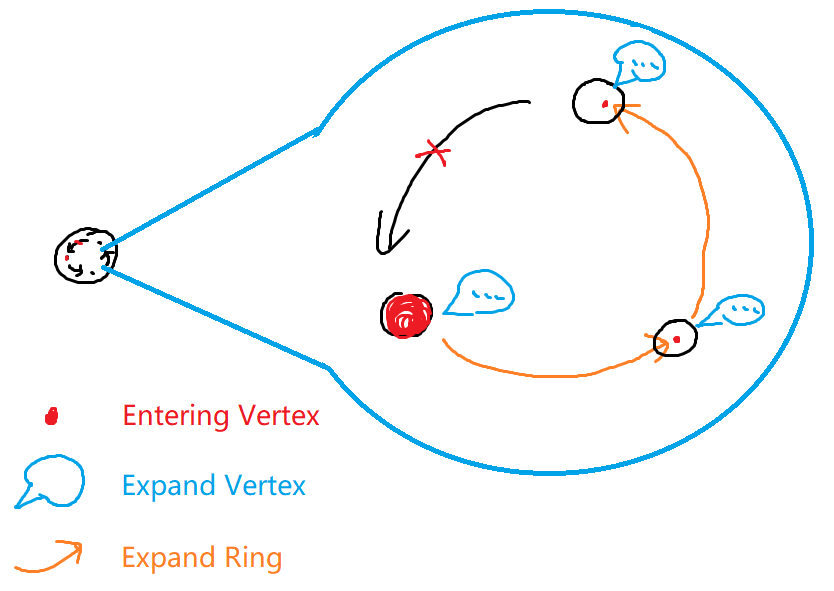
\includegraphics[height=7cm,width=11cm]{figure/figure2.png}
    \caption{graphic explanation for the two functions above}
    \label{2}
\end{figure}

\subsection{Time Complexity Analysis}

Expand part will use the data we calculated in the Contract part once and only once, so the time complexity depends on the Contract part.

In the Contract part, each time we repeat \textbf{step 3.} , we will delete an edge, so we will repeat $m+n=O(m)$ times (note that we added $n$ auxiliary edges). A \textbf{step 3.} cost $O(1)+O(\log n)=O(\log n)$ time. Therefore, the time complexity is $O(m\log n)$.

\section{Data Structures}

\subsection{Lefist Heaps}

A \textbf{Leftist Heap} is a binary heap. Each node in it has a tag $npl$ (Null-Path Length), which means the minimum length from it to a offspring leaf node of it.

A leftist heap node will keep $npl$ of its left son is no less than $npl$ of its right son, and exchange its two sons when this property is broken. Then it will set its own $npl$ to its right son's $npl$ + 1.

There is an interesting lemma about $npl$ and the size of the heap.

\begin{lemma}
    A heap with root's $npl=n$ has at least $2^{n+1}-1$ nodes.
\end{lemma}

\begin{proof}
    This lemma is very easy to proof if we notice another meaning of $npl$: number of full offspring layers.
    
    We know that for the root with $npl=n$, its n-th right offspring has $npl=0$, which means it is a leaf. As each node keeps the property that $npl$ of left son is no less than $npl$ of right son, we know that all the nodes in the same layer has $npl\ge0$, which means at least they all exist. Therefore there are at least $2^{n+1}-1$ nodes.
\end{proof}

\begin{figure}
    \centering
    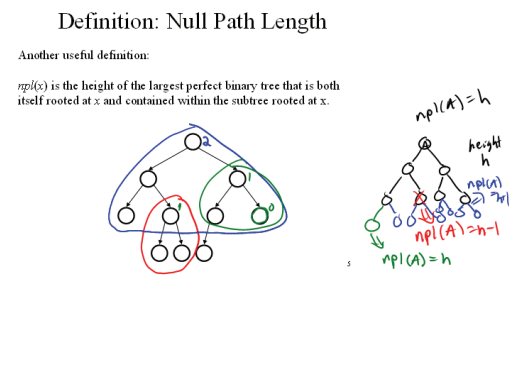
\includegraphics[height=7cm,width=11cm]{figure/figure3.png}
    \caption{a page of Brian Curless's lecture, see References}
    \label{3}
\end{figure}

In other words, $npl=O(\log n)$. Now, let's think how to merge two heaps $a$ and $b$. Obviously, the root with the lower key value in the two roots will be the new root. Let it be $a$, then, we just need to recursively merge $a$'s right son and $b$, then check whether we need to exchange $a$'s two sons.

Each time we recur, $npl_a+npl_b$ will minus $1$, because we always keep one of them unchanged and change the other to its right son. When $npl_a=-1$ or $npl_b=-1$, which means $a$ or $b$ is null, we can just return the other one. Therefore, the merge operation cost $O(\log n)$ time.

Delete-min is very easy since we implemented merge: merge the left son and the right son of the root to be the new root.

When we want to minus a constant from a heap, the construction of the heap will not change, so we can just put a tag on the root. When we try to visit its sons, we first push-down the tags to its sons, so no more time will cost by Minus-constant operation.

Finally, we proved that the leftist heap can finish the three tasks in last section in $O(\log n)$ time.

\subsection{Disjoint Set Unions}

A \textbf{Disjoint Set Union} can tell us which group an element is in and merge two groups. Here we only roughly calculate its time complexity as it is not our bottleneck. For more detailed analysis, see https://oi-wiki.org/ds/dsu/.

Initially, we initialize the DSU with $find[i]=i, size[i]=1$. When querying, we use function $Find(a)$ to repeat $a\leftarrow find[a]$ until $a=find[a]$, and return $a$. When merging, we use function $Merge(a,b)$, which calls $a\leftarrow Find(a)$ and $b\leftarrow Find(b)$ to find their group, and let $size[a]\le size[b]$ (otherwise swap $a$ and $b$), set $find[a]\leftarrow b$ and $size[a]\leftarrow size[a]+size[b]$. Because we always merge the smaller one to the larger one, when we do $a\leftarrow find[a]$ in $Find(a)$, $size[a]$ will at least doubled, and $size[a]\le n$ maintained. Therefore a $Find(a)$ costs $O(\log n)$ time, and so does a $Mereg(a,b)$.

\section{C++ Code}
% settings below are copied from: https://zhuanlan.zhihu.com/p/496764299
\definecolor{mygreen}{rgb}{0,0.6,0}
\definecolor{mygray}{rgb}{0.5,0.5,0.5}
\definecolor{mymauve}{rgb}{0.58,0,0.82}
\lstset{
	backgroundcolor=\color{white},      % choose the background color
	basicstyle=\footnotesize\ttfamily,  % size of fonts used for the code
	columns=fullflexible,
	tabsize=4,
	breaklines=true,               % automatic line breaking only at whitespace
	captionpos=b,                  % sets the caption-position to bottom
	commentstyle=\color{mygreen},  % comment style
	escapeinside={\%*}{*)},        % if you want to add LaTeX within your code
	keywordstyle=\color{blue},     % keyword style
	stringstyle=\color{mymauve}\ttfamily,  % string literal style
	frame=single,
	rulesepcolor=\color{red!20!green!20!blue!20},
	language=C++,
}
\lstset{breaklines}
\lstset{extendedchars=false}
\lstset{numbers=left,numberstyle=\tiny,keywordstyle=\color{blue!70},commentstyle=\color{red!50!green!50!blue!50},rulesepcolor=\color{red!20!green!20!blue!20},escapeinside=``,xleftmargin=-5em,xrightmargin=-5em,aboveskip=1em}
\begin{lstlisting}
    // This code solve the problem in https://www.luogu.com.cn/problem/P4716
    // My submission: https://www.luogu.com.cn/record/105676856
    #include <bits/stdc++.h>
    #define For(_, L, R) for(int _ = L; _ <= R; ++_)
    using namespace std;
    const int MAXN = 400000 + 10;
    const long long INF = 1ll << 40;
    
    typedef pair<pair<long long, long long>, pair<int, int>> Edge; // An edge in the graph
    #define W first.first
    #define W0 first.second
    #define U second.first
    #define V second.second
    #define EDGE(u, v, w) make_pair(make_pair(w, w), make_pair(u, v))
    const Edge EDGENULL = EDGE(0, 0, 0);
    
    template<class T>
    struct Node { // Leftist Tree Node
        Node *ls, *rs;
        int npl; // Null-Path Length
        T val;
        long long tag;
        Node() { ls = rs = NULL; npl = -1; }
        Node(T v): Node() { npl = 0; val = v; tag = 0; }
    };
    template<class T>
    inline void gettag(Node<T> *a, long long gtag) {
        if(a != NULL) {
            a->tag += gtag;
            a->val.W += gtag;
        }
    }
    template<class T>
    inline void pushdown(Node<T> *a) {
        if(a->tag) {
            gettag(a->ls, a->tag);
            gettag(a->rs, a->tag);
            a->tag = 0;
        }
    }
    template<class T>
    Node<T>* merge(Node<T> *a, Node<T> *b) {
        if(a == NULL) return b;
        if(b == NULL) return a;
        if(a->val > b->val) swap(a, b);
        pushdown(a);
        a->rs = merge(a->rs, b);
        if(a->ls == NULL || a->rs->npl > a->ls->npl) swap(a->ls, a->rs);
        a->npl = a->rs == NULL ? 0 : a->rs->npl + 1;
        return a;
    }
    
    int n, m, r;
    
    Node<Edge>* node[MAXN]; // Leftist Tree root of each super-vertex
    Edge in[MAXN]; // In-edge of each node during the contracting process
    int parent[MAXN]; // Each (super-)vertex in which super-vertex
    vector<int> children[MAXN]; // The children of each super-vertex (empty for original vertex)
    inline void addEdge(int u, int v, long long w) {
        node[v] = merge(node[v], new Node<Edge>(EDGE(u, v, w)));
    }
    
    // Use a Union Set to maintain which super-vertex each vertex is in
    int f[MAXN];
    int F(int n) {
        return n == f[n] ? n : f[n] = F(f[n]);
    }
    
    /*
    * To make the code more general, instead of calculate the total value,
    * we want to actually construct the DMST, which will not change our
    * time complexity but cost a little more time.
    */
    Edge tree[MAXN]; // The finally in-edge of each node on DMST
    void expand_ring(int nod);
    
    /*
    * expand_node: We found an original vertex, who is the in-node of 
    * several layers of super-vertices, and the highest layer of which
    * is root. Now we want to calculate the total value of these layers,
    * i.e. the total value inside the super-vertex root.
    */
    void expand_node(int nod, int root) {
        while(nod != root) {
            expand_ring(nod);
            nod = parent[nod];
        }
    }
    
    /*
    * expand_ring: We found a (super-)vertex, who is the in-node of
    * his parent super-vertex. Now we want to calculate the total
    * value of this layer.
    */
    void expand_ring(int nod) {
        for(auto peer : children[parent[nod]])
            if(peer != nod) {
                tree[in[peer].V] = in[peer]; // report an edge
                expand_node(in[peer].V, peer);
            }
    }
    
    int main() {
        /*
        * input
        * The first input n, m, r representing the number of vertices and edges,
        * and the id of the root. The m lines below input u, v, w each line
        * represent an edge E(u, v) = w in the graph.
        */
        cin >> n >> m >> r;
        For(i, 1, m) {
            int u, v, w;
            cin >> u >> v >> w;
            addEdge(u, v, w);
        }
        For(i, 1, n) addEdge(i, i % n + 1, INF); // Make the graph strongly connected
        // initialize
        For(i, 1, n) f[i] = i;
        // contract
        int a = 1; // The (super-)vertex we are considering
        int cnt = n;
        while(node[a] != NULL) { // While LeftistTree[a] is not empty
            // get and delete min
            Edge edge = node[a]->val;
            pushdown(node[a]);
            node[a] = merge(node[a]->ls, node[a]->rs);
            int b = F(edge.U); // b is the super-vertex which u is in
            if(b != a) {
                in[a] = edge;
                if(in[b] == EDGENULL) a = b; // append the link
                    else {
                        int c = ++cnt; // c is the new super-vertex
                        f[c] = c;
                        while(a != c) { // When a == c, we have returned the start point
                            parent[a] = c;
                            f[a] = c;
                            children[c].push_back(a);
                            gettag(node[a], -in[a].W);
                            node[c] = merge(node[c], node[a]);
                            a = F(in[a].U);
                        }
                        a = c;
                    }
            }
        }
        // expand
        expand_node(r, cnt);
        // now, tree[t] for 1 <= t <= n (except tree[r]) contains all edges in DMST
        long long ans = 0;
        For(i, 1, n)
            if(i != r) ans += tree[i].W0;
        if(ans >= INF) cout << -1 << endl;
            else cout << ans << endl;
        return 0;
    }
\end{lstlisting}

\section{Extensions}

What if we are not given a root $r$ but required to find an optimal $r$ so that the total cost of our MDST is minimized? We can add a virture super source vertex $s$, add edges $(s,1),(s,2),...,(s,n)$ with weight $INF$, and again make the whole graph strongly connected. Then, use the algorithm above to solve the problem with the new graph and root $s$. If the total cost is greater than $2\times INF$, then there is no legal solution. Otherwise, we ignore the only edge beginning from $s$, and the other edges form the optimal MDST.

\newpage

\renewcommand\refname{References}
\begin{thebibliography}{99}
    \bibitem[Uri Zwick(2013)]{MDST} Directed Minimum Spanning Trees

    https://www.cs.princeton.edu/courses/archive/spring13/cos528/directed-mst-1.pdf
    
    \bibitem[Brian Curless(2008)]{LH} Lefist Heaps

    https://courses.cs.washington.edu/courses/cse326/08sp/lectures/markup/05-leftist-heaps-markup.pdf
\end{thebibliography}

\end{document}
